\noindent\markforreview
\vspace{1em}


Hector used a tool called an auger to remove corn from a storage bin at a constant rate. The bin contained 24,000 bushels of corn when Hector began to use the auger. After 5 hours of using the auger, 19,350 bushels of corn remained in the bin. If the auger continues to remove corn at this rate, what is the total number of hours Hector will have been using the auger when 12,840 bushels of corn remain in the bin?

\vspace{0.75em}

\choicebox{A}{3}
\choicebox{B}{7}
\choicebox{C}{8}
\choicebox{D}{12}




\vspace{2em}

\noindent\markforreview

\vspace{1em}

Alan drives an average of 100 miles each week. His car can travel an average of 25 miles per gallon of gasoline. Alan would like to reduce his weekly expenditure on gasoline by \$5. Assuming gasoline costs \$4 per gallon, which equation can Alan use to determine how many fewer average miles, \( m \), he should drive each week?

\vspace{0.75em}

\choicebox{A}{$\frac{25}{4}m = 95$}
\choicebox{B}{$\frac{25}{4}m = 5$}
\choicebox{C}{$\frac{4}{25}m = 95$}
\choicebox{D}{$\frac{4}{25}m = 5$}




\newpage

\noindent\markforreview
\vspace{1em}

How many solutions does the equation \( 10(15x - 9) = -15(6 - 10x) \) have?

\vspace{0.75em}

\choicebox{A}{Exactly one}
\choicebox{B}{Exactly two}
\choicebox{C}{Infinitely many}
\choicebox{D}{Zero}



\vspace{2em}

\noindent\markforreview

In the given equation, \( k \) is a constant. The equation has no solution. What is the value of \( k \)?

\[
3(kx + 13) = \frac{48}{17}x + 36
\]





\newpage
\noindent\markforreview

\vspace{1em}

A certain product costs a company \$65 to make. The product is sold by a salesperson who earns a commission that is equal to 20\% of the sales price of the product. The profit the company makes for each unit is equal to the sales price minus the combined cost of making the product and the commission. If the sales price of the product is \$100, which of the following equations gives the number of units, \( u \), of the product the company sold to make a profit of \$6{,}840?

\vspace{0.75em}

\choicebox{A}{\( (100(1 - 0.2) - 65)u = 6840 \)}
\choicebox{B}{\( (100 - 65)(1 - 0.8)u = 6840 \)}
\choicebox{C}{\( 0.8(100) - 65u = 6840 \)}
\choicebox{D}{\( 0.2(100) + 65)u = 6840 \)}

\vspace{2em}

\noindent\markforreview

\vspace{1em}

In the given equation, \( k \) and \( n \) are constants and \( n > 1 \). The equation has no solution. What is the value of \( k \)?

\[
2(kx - n) = -\frac{28}{15}x - \frac{36}{19}
\]





\newpage
\noindent\markforreview

\vspace{1em}

What value of \( t \) is the solution to the given equation?

\[
5(t + 3) - 7(t + 3) = 38
\]


\vspace{2em}

\noindent\markforreview

\vspace{1em}

\begin{center}
\textbf{Townsend Realty Group Investments}

\vspace{0.75em}
\renewcommand{\arraystretch}{1.3}
\begin{tabular}{|l|c|c|}
\hline
\textbf{Property address} & \textbf{Purchase price (dollars)} & \textbf{Monthly rental price (dollars)} \\
\hline
Clearwater Lane & 128{,}000 & 950 \\
Driftwood Drive & 176{,}000 & 1{,}310 \\
Edgemont Street & 70{,}000 & 515 \\
Glenview Street & 140{,}000 & 1{,}040 \\
Hamilton Circle & 450{,}000 & 3{,}365 \\
\hline
\end{tabular}
\end{center}

\vspace{1em}

The Townsend Realty Group invested in the five different properties listed in the table above. The table shows the amount, in dollars, the company paid for each property and the corresponding monthly rental price, in dollars, the company charges for the property at each of the five locations.

Townsend Realty purchased the Glenview Street property and received a 40\% discount off the original price along with an additional 20\% off the discounted price for purchasing the property in cash. Which of the following best approximates the original price, in dollars, of the Glenview Street property?

\vspace{0.75em}

\choicebox{A}{\$350{,}000}
\choicebox{B}{\$291{,}700}
\choicebox{C}{\$233{,}300}
\choicebox{D}{\$175{,}000}

\newpage
\noindent\markforreview

\vspace{1em}

Each side of a 30-sided polygon has one of three lengths. The number of sides with length 8 \textbf{centimeters (cm)} is 5 times the number of sides \( n \) with length 3 cm. There are 6 sides with length 4 cm. Which equation must be true for the value of \( n \)?

\vspace{0.75em}

\choicebox{A}{$5n + 6 = 30$}
\choicebox{B}{$6n + 6 = 30$}
\choicebox{C}{$8n + 3n + 4n = 30$}
\choicebox{D}{$8(5n) + 3n + 4(6) = 30$}

\vspace{2em}

\noindent\markforreview

\vspace{1em}

In the given equation, \( p \) is a constant. The equation has no solution. What is the value of \( p \)?

\[
-3x + 21px = 84
\]

\vspace{0.75em}

\choicebox{A}{$p = 0$}
\choicebox{B}{$p = \frac{1}{7}$}
\choicebox{C}{$p = \frac{4}{3}$}
\choicebox{D}{$p = 4$}


\newpage
\noindent\markforreview

\vspace{1em}

If \( \frac{x + 6}{3} = \frac{x + 6}{13} \), the value of \( x + 6 \) is between which of the following pairs of values?

\vspace{0.75em}

\choicebox{A}{\(-7\) and \(-3\)}
\choicebox{B}{\(-2\) and 2}
\choicebox{C}{2 and 7}
\choicebox{D}{8 and 13}

\vspace{2em}


\noindent\markforreview

\vspace{1em}

The equation \( 9x + 5 = a(x + b) \), where \( a \) and \( b \) are constants, has no solutions.  
Which of the following must be true?

\begin{itemize}
  \item[I.] \( a = 9 \)
  \item[II.] \( b = 5 \)
  \item[III.] \( b \ne \frac{5}{9} \)
\end{itemize}

\vspace{0.75em}

\choicebox{A}{None}
\choicebox{B}{I only}
\choicebox{C}{I and II only}
\choicebox{D}{I and III only}

\newpage
\noindent\markforreview

\vspace{1em}

A science teacher is preparing the 5 stations of a science laboratory. Each station will have either Experiment A materials or Experiment B materials, but not both. Experiment A requires 6 teaspoons of salt, and Experiment B requires 4 teaspoons of salt. If \( x \) is the number of stations that will be set up for Experiment A and the remaining stations will be set up for Experiment B, which of the following expressions represents the total number of teaspoons of salt required?

\vspace{0.75em}

\choicebox{A}{$5x$}
\choicebox{B}{$10x$}
\choicebox{C}{$2x + 20$}
\choicebox{D}{$10x + 20$}

\newpage
\subsection*{1.2 Linear Function}
\setcounter{questionnum}{0}


\noindent\markforreview

\vspace{1em}

A window repair specialist charges \textbf{\$220} for the first two hours of repair plus an hourly fee for each additional hour. The total cost for 5 hours of repair is \textbf{\$400}. Which function \( f \) gives the total cost, in dollars, for \( x \) hours of repair, where \( x \geq 2 \)?

\vspace{0.75em}

\choicebox{A}{$f(x) = 60x + 100$}
\choicebox{B}{$f(x) = 60x + 220$}
\choicebox{C}{$f(x) = 80x$}
\choicebox{D}{$f(x) = 80x + 220$}

\vspace{2em}
\noindent\markforreview

\vspace{1em}

An economist modeled the demand \( Q \) for a certain product as a linear function of the selling price \( P \). The demand was 20{,}000 units when the selling price was \$40 per unit, and the demand was 15{,}000 units when the selling price was \$60 per unit. Based on the model, what is the demand, in units, when the selling price is \$55 per unit?

\vspace{0.75em}

\choicebox{A}{16{,}250}
\choicebox{B}{16{,}500}
\choicebox{C}{16{,}750}
\choicebox{D}{17{,}500}

\newpage
\noindent\markforreview

\vspace{1em}

The cost of renting a backhoe for up to 10 days is \$270 for the first day and \$135 for each additional day. Which of the following equations gives the cost \( y \), in dollars, of renting the backhoe for \( x \) days, where \( x \) is a positive integer and \( x \leq 10 \)?

\vspace{0.75em}

\choicebox{A}{$y = 270x - 135$}
\choicebox{B}{$y = 270x + 135$}
\choicebox{C}{$y = 135x + 270$}
\choicebox{D}{$y = 135x + 135$}

\vspace{2em}
\noindent\markforreview

\vspace{1em}

The function \( F \) gives the temperature, in degrees Fahrenheit, that corresponds to a temperature of \( x \) kelvins. If a temperature increased by 9.10 kelvins, by how much did the temperature increase, in degrees Fahrenheit?

\[
F(x) = \frac{9}{5}(x - 273.15) + 32
\]

\vspace{0.75em}

\choicebox{A}{16.38}
\choicebox{B}{48.38}
\choicebox{C}{475.29}
\choicebox{D}{507.29}


\newpage
\noindent\markforreview

\vspace{1em}

The functions \( f \) and \( g \) are defined as \( f(x) = \frac{1}{4}x - 9 \) and \( g(x) = \frac{3}{4}x + 21 \). If the function \( h \) is defined as \( h(x) = f(x) + g(x) \), what is the \( x \)-coordinate of the \( x \)-intercept of the graph of \( y = h(x) \) in the \( xy \)-plane?



\vspace{2em}
\noindent\markforreview

\vspace{1em}

According to data provided by the US Department of Energy, the average price per gallon of regular gasoline in the United States from September 1, 2014, to December 1, 2014, is modeled by the function \( F \) defined below, where \( F(x) \) is the average price per gallon \( x \) months after September 1.

\[
F(x) = 2.74 - 0.19(x - 3)
\]

The constant 2.74 in this function estimates which of the following?

\vspace{0.75em}

\choicebox{A}{The average monthly decrease in the price per gallon}
\choicebox{B}{The difference in the average price per gallon from September 1, 2014, to December 1, 2014}
\choicebox{C}{The average price per gallon on September 1, 2014}
\choicebox{D}{The average price per gallon on December 1, 2014}



\newpage
\noindent\markforreview

\vspace{1em}

For the linear function \( f \), the table shows three values of \( x \) and their corresponding values of \( f(x) \). Function \( f \) is defined by \( f(x) = ax + b \), where \( a \) and \( b \) are constants. What is the value of \( a - b \)?

\begin{center}
\begin{tabular}{|c|c|}
\hline
$x$ & $f(x)$ \\
\hline
1 & -64 \\
2 & 0 \\
3 & 64 \\
\hline
\end{tabular}
\end{center}

\vspace{0.75em}

\choicebox{A}{$-64$}
\choicebox{B}{$62$}
\choicebox{C}{$128$}
\choicebox{D}{$192$}

\vspace{2em}

\noindent\markforreview

\vspace{1em}

Oil and gas production in a certain area dropped from 4 million barrels in 2000 to 1.9 million barrels in 2013. Assuming that the oil and gas production decreased at a constant rate, which of the following linear functions \( f \) best models the production, in millions of barrels, \( t \) years after the year 2000?

\vspace{0.75em}

\choicebox{A}{$f(t) = \frac{21}{130}t + 4$}
\choicebox{B}{$f(t) = \frac{19}{130}t + 4$}
\choicebox{C}{$f(t) = -\frac{21}{130}t + 4$}
\choicebox{D}{$f(t) = -\frac{19}{130}t + 4$}

\newpage



\noindent\markforreview

\vspace{1em}

One gallon of paint will cover 220 square feet of a surface. A room has a total wall area of \( w \) square feet. Which equation represents the total amount of paint \( P \), in gallons, needed to paint the walls of the room twice?

\vspace{0.75em}

\choicebox{A}{$P = \frac{w}{110}$}
\choicebox{B}{$P = 440w$}
\choicebox{C}{$P = \frac{w}{220}$}
\choicebox{D}{$P = 220w$}

\vspace{2em}

\noindent\markforreview

\vspace{1em}

The function \( F \) gives the temperature, in degrees Fahrenheit, that corresponds to a temperature of \( x \) kelvins. If a temperature increased by 2.10 kelvins, by how much did the temperature increase, in degrees Fahrenheit?

\[
F(x) = \frac{9}{5}(x - 273.15) + 32
\]

\vspace{0.75em}

\choicebox{A}{$3.78$}
\choicebox{B}{$35.78$}
\choicebox{C}{$487.89$}
\choicebox{D}{$519.89$}

\newpage



\noindent\markforreview

\vspace{1em}

The table above shows some values of \( x \) and their corresponding values \( f(x) \) for the linear function \( f \). What is the \( x \)-intercept of the graph of \( y = f(x) \) in the \( xy \)-plane?

\begin{center}
\begin{tabular}{|c|c|c|c|c|}
\hline
$x$ & -11 & -10 & -9 & -8 \\
\hline
$f(x)$ & 21 & 18 & 15 & 12 \\
\hline
\end{tabular}
\end{center}

\vspace{0.75em}

\choicebox{A}{\((-3, 0)\)}
\choicebox{B}{\((-4, 0)\)}
\choicebox{C}{\((-9, 0)\)}
\choicebox{D}{\((-12, 0)\)}


\newpage
\noindent\markforreview

\vspace{1em}

\begin{center}
\begin{tabular}{|l|c|c|}
\hline
\textbf{Macronutrient} & \textbf{Food calories} & \textbf{Kilojoules} \\
\hline
Protein     & 4.0 & 16.7 \\
Fat         & 9.0 & 37.7 \\
Carbohydrate & 4.0 & 16.7 \\
\hline
\end{tabular}
\end{center}

The table above gives the typical amounts of energy per gram, expressed in both food calories and kilojoules, of the three macronutrients in food. If the 180 food calories in a granola bar come entirely from \( p \) grams of protein, \( f \) grams of fat, and \( c \) grams of carbohydrate, which of the following expresses \( f \) in terms of \( p \) and \( c \)?

\vspace{0.75em}

\choicebox{A}{$f = 20 + \frac{4}{9}(p + c)$}
\choicebox{B}{$f = 20 - \frac{4}{9}(p + c)$}
\choicebox{C}{$f = 20 - \frac{4}{9}p - c$}
\choicebox{D}{$f = 20 + \frac{9}{4}(p + c)$}

\vspace{2em}
\newpage
\noindent\markforreview

\vspace{1em}

An object hangs from a spring. The formula \( \ell = 30 + 2w \) relates the length \( \ell \), in centimeters, of the spring to the weight \( w \), in newtons, of the object. Which of the following describes the meaning of the 2 in this context?

\vspace{0.75em}

\choicebox{A}{The length, in centimeters, of the spring with no weight attached}
\choicebox{B}{The weight, in newtons, of an object that will stretch the spring 30 centimeters}
\choicebox{C}{The increase in the weight, in newtons, of the object for each one-centimeter increase in the length of the spring}
\choicebox{D}{The increase in the length, in centimeters, of the spring for each one-newton increase in the weight of the object}


\vspace{2em}
\noindent\markforreview

\vspace{1em}

For the function \( f \), if \( f(3x) = x - 6 \) for all values of \( x \), what is the value of \( f(6) \)?

\vspace{0.75em}

\choicebox{A}{$-6$}
\choicebox{B}{$-4$}
\choicebox{C}{$0$}
\choicebox{D}{$2$}



\newpage
\noindent\markforreview

\vspace{1em}

For groups of 25 or more people, a museum charges \$21 per person for the first 25 people and \$14 for each additional person. Which function \( f \) gives the total charge, in dollars, for a tour group with \( n \) people, where \( n \geq 25 \)?

\vspace{0.75em}

\choicebox{A}{$f(n) = 14n + 175$}
\choicebox{B}{$f(n) = 14n + 525$}
\choicebox{C}{$f(n) = 35n - 350$}
\choicebox{D}{$f(n) = 14n + 21$}


\newpage

\subsection*{1.3 Linear Equation in Two Varibles}

\vspace{0.5em}

\setcounter{questionnum}{0}

\noindent\markforreview

\vspace{1em}

The table gives the coordinates of two points on a line in the $xy$-plane. The $y$-intercept of the line is $(k - 5, b)$, where $k$ and $b$ are constants. What is the value of $b$?

\[
\begin{array}{c|c}
x & y \\
\hline
k & 13 \\
k + 7 & -15 \\
\end{array}
\]

\vspace{0.75em}


\vspace{2em}

\noindent\markforreview

\vspace{1em}

The graph of the equation $ax + ky = 6$ is a line in the $xy$-plane, where $a$ and $k$ are constants. If the line contains the points $(-2, -6)$ and $(0, -3)$, what is the value of $k$?

\vspace{0.75em}

\choicebox{A}{$-2$}
\choicebox{B}{$-1$}
\choicebox{C}{$2$}
\choicebox{D}{$3$}

\newpage
\noindent\markforreview

\vspace{1em}

For line $h$, the table shows three values of $x$ and their corresponding values of $y$. Line $k$ is the result of translating line $h$ down 5 units in the $xy$-plane. What is the $x$-intercept of line $k$?

\[
\begin{array}{c|c}
x & y \\
\hline
18 & 130 \\
23 & 160 \\
26 & 178 \\
\end{array}
\]

\vspace{0.75em}

\choicebox{A}{$\left( -\frac{26}{3}, 0 \right)$}
\choicebox{B}{$\left( -\frac{9}{2}, 0 \right)$}
\choicebox{C}{$\left( -\frac{11}{3}, 0 \right)$}
\choicebox{D}{$\left( -\frac{17}{6}, 0 \right)$}

\vspace{2em}

\noindent\markforreview

\vspace{1em}

A certain apprentice has enrolled in 85 hours of training courses. The equation $10x + 15y = 85$ represents this situation, where $x$ is the number of on-site training courses and $y$ is the number of online training courses this apprentice has enrolled in. How many more hours does each online training course take than each on-site training course?

\newpage
\noindent\markforreview

\vspace{1em}

Line $p$ is defined by $4y + 8x = 6$. Line $r$ is perpendicular to line $p$ in the $xy$-plane. What is the slope of line $r$?


\vspace{15em}

\noindent\markforreview

\vspace{1em}

In the $xy$-plane, line $k$ intersects the $y$-axis at the point $(0, -6)$ and passes through the point $(2, 2)$. If the point $(20, w)$ lies on line $k$, what is the value of $w$?


\vspace{15em}

\noindent\markforreview

\vspace{1em}

In the $xy$-plane, line $\ell$ passes through the point $(0, 0)$ and is parallel to the line represented by the equation $y = 8x + 2$. If line $\ell$ also passes through the point $(3, d)$, what is the value of $d$?

\vspace{2em}

\newpage
\noindent\markforreview

\vspace{1em}
\begin{center}
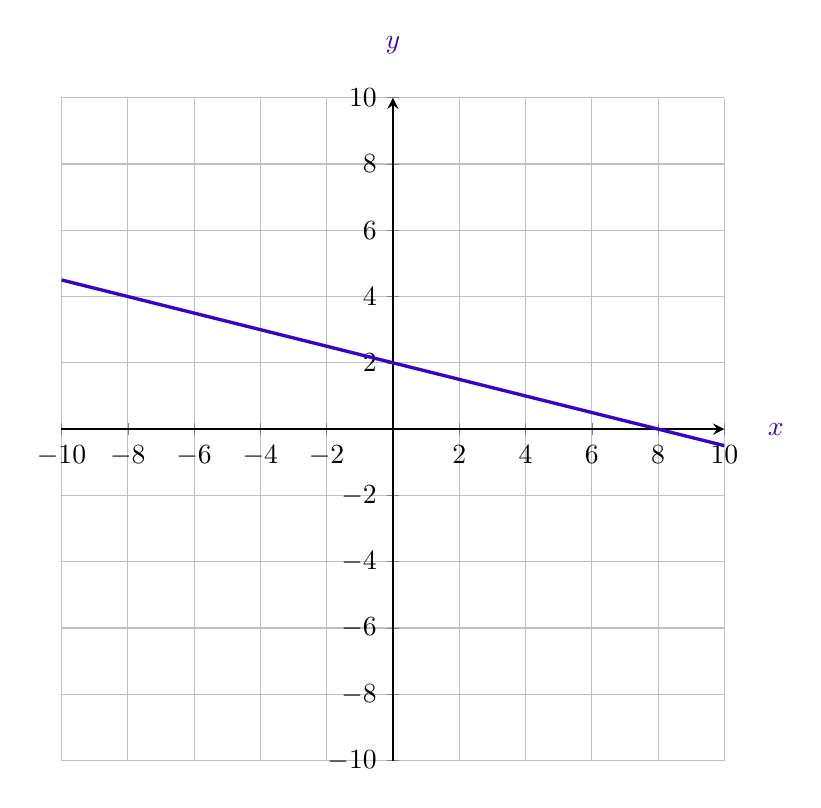
\begin{tikzpicture}
  \begin{axis}[
    axis lines=middle,
    % 紫蓝色刻度线
    xmin=-10, xmax=10,
    ymin=-10, ymax=10,
    xtick={-10,-8,...,10},
    ytick={-10,-8,...,10},
    grid=both,
    width=10cm,
    height=10cm,
    enlargelimits=false,
    xlabel={$x$}, ylabel={$y$},
    every axis x label/.style={
      at={(ticklabel* cs:1.05)}, anchor=west, color=purple!30!blue, font=\bfseries
    },
    every axis y label/.style={
      at={(ticklabel* cs:1.05)}, anchor=south, color=purple!30!blue, font=\bfseries
    },
    domain=-10:10,
    samples=2,
    thick
  ]
    \addplot [purple!30!blue, very thick] {-0.25*x + 2};
  \end{axis}
\end{tikzpicture}
\end{center}
\vspace{0.75em}

The graph of \( y = f(x) + 14 \) is shown. Which equation defines function \( f \)?

\vspace{0.75em}

\choicebox{A}{$f(x) = -\frac{1}{4}x - 12$}
\choicebox{B}{$f(x) = -\frac{1}{4}x + 16$}
\choicebox{C}{$f(x) = -\frac{1}{4}x + 2$}
\choicebox{D}{$f(x) = -\frac{1}{4}x - 14$}


\newpage


\noindent\markforreview

\vspace{1em}

Keenan made \textbf{32} cups of vegetable broth. Keenan then filled \( x \) small jars and \( y \) large jars with all the vegetable broth he made. The equation \( 3x + 5y = 32 \) represents this situation. Which is the best interpretation of \( 5y \) in this context?

\vspace{0.75em}

\choicebox{A}{The number of large jars Keenan filled}
\choicebox{B}{The number of small jars Keenan filled}
\choicebox{C}{The total number of cups of vegetable broth in the large jars}
\choicebox{D}{The total number of cups of vegetable broth in the small jars}

\newpage

\noindent\markforreview

\vspace{1em}

\[ax+by=b\]

In the equation above, \( a \) and \( b \) are constants and \( 0 < a < b \). Which of the following could represent the graph of the equation in the \( xy \)-plane?

\textbf{For each length of the square, it counts 0.5}




\choicebox{A}{%
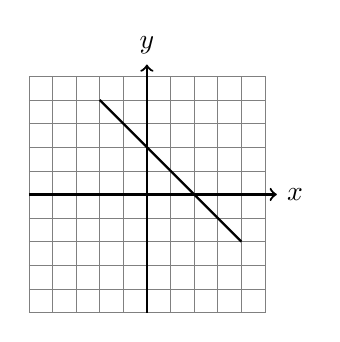
\begin{tikzpicture}[scale=0.3]
  \draw[step=1cm,gray,very thin] (-5,-5) grid (5,5);
  \draw[->,thick] (-5,0) -- (5.5,0) node[right] {$x$};
  \draw[->,thick] (0,-5) -- (0,5.5) node[above] {$y$};
  \draw[thick] (-2,4) -- (4,-2);
\end{tikzpicture}}


\choicebox{B}{%
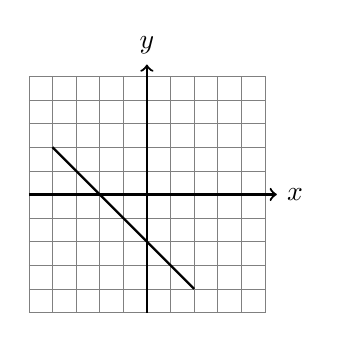
\begin{tikzpicture}[scale=0.3]
  \draw[step=1cm,gray,very thin] (-5,-5) grid (5,5);
  \draw[->,thick] (-5,0) -- (5.5,0) node[right] {$x$};
  \draw[->,thick] (0,-5) -- (0,5.5) node[above] {$y$};
  \draw[thick] (-4,2) -- (2,-4);
\end{tikzpicture}}

\choicebox{C}{%
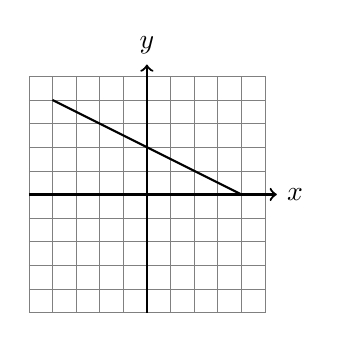
\begin{tikzpicture}[scale=0.3]
  \draw[step=1cm,gray,very thin] (-5,-5) grid (5,5);
  \draw[->,thick] (-5,0) -- (5.5,0) node[right] {$x$};
  \draw[->,thick] (0,-5) -- (0,5.5) node[above] {$y$};
  \draw[thick] (4,0) -- (-4,4);
\end{tikzpicture}}

\choicebox{D}{%
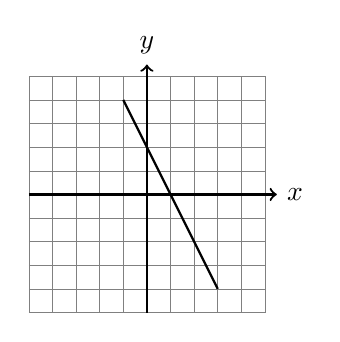
\begin{tikzpicture}[scale=0.3]
  \draw[step=1cm,gray,very thin] (-5,-5) grid (5,5);
  \draw[->,thick] (-5,0) -- (5.5,0) node[right] {$x$};
  \draw[->,thick] (0,-5) -- (0,5.5) node[above] {$y$};
  \draw[thick] (3,-4) -- (-1,4);
\end{tikzpicture}}


\newpage
\noindent\markforreview

\vspace{1em}

The points plotted in the coordinate plane above represent the possible numbers of wallflowers and cornflowers that someone can buy at the Garden Store in order to spend exactly \$24.00 total on the two types of flowers. The price of each wallflower is the same and the price of each cornflower is the same. What is the price, in dollars, of 1 cornflower?

\begin{center}
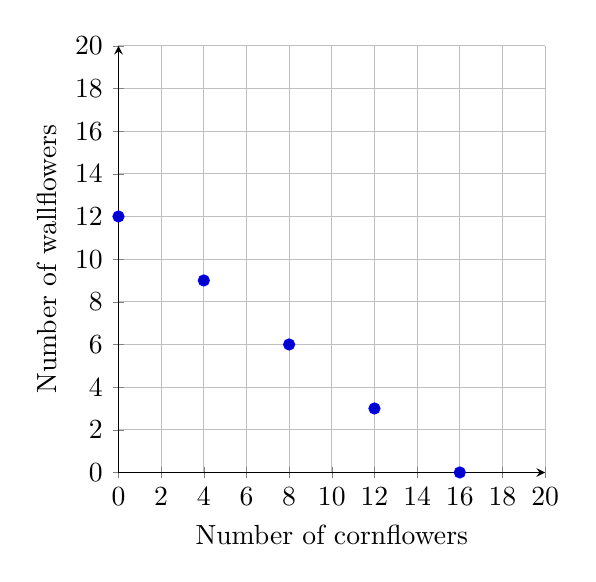
\begin{tikzpicture}
  \begin{axis}[
    width=7cm, height=7cm,
    grid=major,
    xmin=0, xmax=20,
    ymin=0, ymax=20,
    xlabel=Number of cornflowers,
    ylabel=Number of wallflowers,
    xtick={0,2,...,20},
    ytick={0,2,...,20},
    enlargelimits=false,
    axis lines=left,
    every axis plot/.append style={only marks, mark=*}
  ]
  \addplot coordinates {
    (0,12)
    (4,9)
    (8,6)
    (12,3)
    (16,0)
  };
  \end{axis}
\end{tikzpicture}
\end{center}

\vspace{2em}
\noindent\markforreview

\vspace{1em}

The graph of \( 7x + 2y = -31 \) in the \( xy \)-plane has an \( x \)-intercept at \( (a, 0) \) and a \( y \)-intercept at \( (0, b) \), where \( a \) and \( b \) are constants. What is the value of \( \frac{b}{a} \)?

\vspace{0.75em}

\choicebox{A}{$-\frac{7}{2}$}
\choicebox{B}{$-\frac{2}{7}$}
\choicebox{C}{$\frac{2}{7}$}
\choicebox{D}{$\frac{7}{2}$}

\newpage
\noindent\markforreview

\vspace{1em}

Line $\ell$ in the $xy$-plane is perpendicular to the line with equation $x = 2$. What is the slope of line $\ell$?

\vspace{0.75em}

\choicebox{A}{$0$}
\choicebox{B}{$\dfrac{1}{2}$}
\choicebox{C}{$-2$}
\choicebox{D}{The slope of line $\ell$ is undefined.}


\vspace{5em}
\noindent\markforreview

\vspace{1em}

The graph of \( 9x - 10y = 19 \) is translated down 4 units in the xy-plane. What is the x-coordinate of the x-intercept of the resulting graph?


\vspace{5em}
\newpage
\noindent\markforreview

\vspace{1em}

The table above shows the coordinates of three points on a line in the xy-plane, where \( k \) and \( n \) are constants. If the slope of the line is 2, what is the value of \( k + n \)?

\[
\begin{array}{c|c}
x & y \\
\hline
3 & 7 \\
k & 11 \\
12 & n \\
\end{array}
\]

\vspace{5em}

\noindent\markforreview

\vspace{1em}

In the given pair of equations, \( a \) and \( b \) are constants. The graph of this pair of equations in the xy-plane is a pair of perpendicular lines. Which of the following pairs of equations also represents a pair of perpendicular lines?

\[
\begin{aligned}
5x + 7y = 1 \\
ax + by = 1 \\
\end{aligned}
\]

\vspace{0.75em}

\choicebox{A}{\(10x + 7y = 1 \quad\) and  \(2ax + 5by = 1\)}
\choicebox{B}{\(10x + 7y = 1 \quad\) and  \(ax + 2by = 1\)}
\choicebox{C}{\(10x + 7y = 1 \quad\) and  \(2ax + by = 1\)}
\choicebox{D}{\(5x - 7y = 1 \quad\) and  \(ax + by = 1\)}

\newpage

\noindent\markforreview

\vspace{1em}

At a school fair, students can win colored tokens that are worth a different number of points depending on the color. One student won \( G \) green tokens and \( R \) red tokens worth a total of 380 points. The given equation represents this situation. How many more points is a red token worth than a green token?

\[
5G + 45R = 380
\]

\vspace{2em}
\noindent\markforreview

\vspace{1em}

To earn money for college, Avery works two part-time jobs: A and B. She earns \$10 per hour working at job A and \$20 per hour working at job B. In one week, Avery earned a total of \( s \) dollars for working at the two part-time jobs. The graph below represents all possible combinations of numbers of hours Avery could have worked at the two jobs to earn \( s \) dollars. What is the value of \( s \)?

\begin{center}
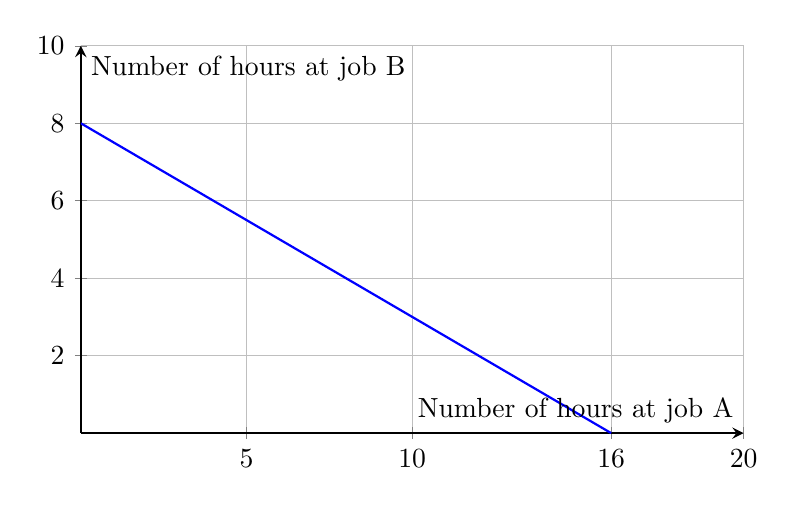
\begin{tikzpicture}
  \begin{axis}[
    width=10cm,
    height=6.5cm,
    xmin=0, xmax=20,
    ymin=0, ymax=10,
    axis lines=middle,
    xlabel={Number of hours at job A},
    ylabel={Number of hours at job B},
    xtick={0,5,10,16, 20},
    ytick={0,2,4,6,8,10},
    grid=major,
    thick
  ]
    % Plot the line y = 10 - 0.5x
    \addplot[
      domain=0:20,
      samples=100,
      thick,
      color=blue
    ] coordinates{(0,8)
    (16,0)};
  \end{axis}
\end{tikzpicture}
\end{center}




\choicebox{A}{128}
\choicebox{B}{160}
\choicebox{C}{200}
\choicebox{D}{320}

\newpage
\noindent\markforreview

\vspace{1em}

The line with the equation \( \frac{4}{5}x + \frac{1}{3}y = 1 \) is graphed in the \( xy \)-plane.

\vspace{2mm}
What is the x-coordinate of the x-intercept of the line?


\vspace{2em}

\noindent\markforreview

\vspace{1em}

\begin{center}
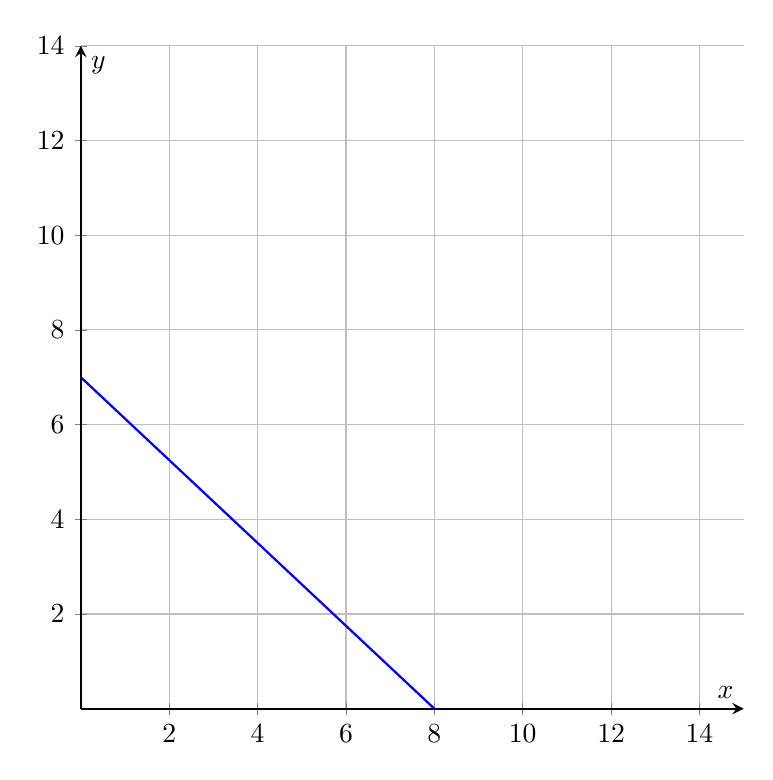
\begin{tikzpicture}
  \begin{axis}[
    width=10cm,
    height=10cm,
    xmin=0, xmax=15,
    ymin=0, ymax=14,
    axis lines=middle,
    xlabel={$x$},
    ylabel={$y$},
    xtick={0,2,...,14},
    ytick={0,2,...,14},
    grid=major,
    thick
  ]
    \addplot[domain=0:10, samples=2, thick, color=blue] coordinates{(0,7)
    (8,0)}; % Equation: y = -x + 10
  \end{axis}
\end{tikzpicture}
\end{center}

The point with coordinates $(d, 4)$ lies on the line shown. What is the value of $d$?

\vspace{0.75em}

\choicebox{A}{$\frac{7}{2}$}
\choicebox{B}{$\frac{26}{7}$}
\choicebox{C}{$\frac{24}{7}$}
\choicebox{D}{$\frac{27}{8}$}

\vspace{2em}

\noindent\markforreview

\vspace{1em}

In the $xy$-plane, line $k$ is defined by $x + y = 0$. Line $j$ is perpendicular to line $k$, and the $y$-intercept of line $j$ is $(0,3)$. Which of the following is an equation of line $j$?

\vspace{0.75em}

\choicebox{A}{$x + y = 3$}
\choicebox{B}{$x + y = -3$}
\choicebox{C}{$x - y = 3$}
\choicebox{D}{$x - y = -3$}


\vspace{2em}

\noindent\markforreview

\vspace{1em}

How many liters of a 25\% saline solution must be added to 3 liters of a 10\% saline solution to obtain a 15\% saline solution?


\newpage
\subsection*{1.4 System of Two Linear Equations In Two Variables }
\vspace{0.5em}

\setcounter{questionnum}{0}

\noindent\markforreview

\vspace{0.5em}
\[
\begin{aligned}
-x + y = -3.5 \\ 
x + 3y = 9.5
\end{aligned}
  \]


If $(x, y)$ satisfies the system of equations above, what is the value of $y$?


\vspace{5em}
\noindent\markforreview

\vspace{0.5em}

\[
\begin{aligned}
\frac{3}{2}y - \frac{1}{4}x &= \frac{2}{3}-\frac{3}{2}y \\
\frac{1}{2}x + \frac{3}{2} &= py + \frac{9}{2}
\end{aligned}
\]

In the given system of equations, $p$ is a constant. If the system has no solution, what is the value of $p$?


\vspace{5em}
\noindent\markforreview

\vspace{0.5em}

\[
\begin{aligned}
4x - 6y &= 10y + 2 \\
ty &= \frac{1}{2} + 2x
\end{aligned}
\]

In the given system of equations, $t$ is a constant. If the system has no solution, what is the value of $t$?

\newpage
\noindent\markforreview

\vspace{1em}

During a month, Morgan ran $r$ miles at 5 miles per hour and biked $b$ miles at 10 miles per hour. She ran and biked a total of 200 miles that month, and she biked for twice as many hours as she ran. What is the total number of miles that Morgan biked during the month?

\vspace{0.75em}

\choicebox{A}{80}
\choicebox{B}{100}
\choicebox{C}{120}
\choicebox{D}{160}


\vspace{2em}
\noindent\markforreview

\vspace{1em}

In the system of equations below, \( a \) and \( c \) are constants.
\[
\frac{1}{2}x + \frac{1}{3}y = \frac{1}{6}
\]
\[
ax + y = c
\]
If the system of equations has an infinite number of solutions \( (x, y) \), what is the value of \( a \)?

\vspace{0.75em}

\choicebox{A}{$-\dfrac{1}{2}$}
\choicebox{B}{$0$}
\choicebox{C}{$\dfrac{1}{2}$}
\choicebox{D}{$\dfrac{3}{2}$}

\newpage
\noindent\markforreview

\vspace{1em}

\[
y = 4x + 1
\]
\[
4y = 15x - 8
\]
The solution to the given system of equations is \( (x, y) \). What is the value of \( x - y \)?

\vspace{5em}



\noindent\markforreview

\vspace{1em}

\[
\begin{aligned}
7x - 5y &= 4 \\
4x - 8y &= 9
\end{aligned}
\]
If \( (x, y) \) is the solution to the system of equations above, what is the value of \( 3x + 3y \)?

\vspace{0.75em}

\choicebox{A}{$-13$}
\choicebox{B}{$-5$}
\choicebox{C}{$5$}
\choicebox{D}{$13$}


\newpage

\noindent\markforreview

\vspace{1em}

In the given system of equations, \( r \) is a constant. If the system has no solution, what is the value of \( r \)?

\[
\begin{aligned}
48x - 72y &= 30y + 24 \\
ry &= \frac{1}{6} - 16x
\end{aligned}
\]

\vspace{5em}
\noindent\markforreview

\vspace{1em}

The solution to the given system of equations is \( (x, y) \). What is the value of \( y \)?

\[
\begin{aligned}
24x + y &= 48 \\
6x + y &= 72
\end{aligned}
\]

\vspace{5em}
\noindent\markforreview

\vspace{1em}

A movie theater sells two types of tickets, adult tickets for \$12 and child tickets for \$8. If the theater sold 30 tickets for a total of \$300, how much, in dollars, was spent on adult tickets? (Disregard the \$ sign when gridding your answer.)

\newpage
\noindent\markforreview

\vspace{1em}

The solution to the given system of equations is \( (x, y) \). What is the value of \( xy \)?

\[
\begin{aligned}
5x + 14y &= 45 \\
10x + 7y &= 27
\end{aligned}
\]

\vspace{2em}

\noindent\markforreview

\vspace{1em}

In the system of equations below, \( c \) is a constant. If the system has no solution, what is the value of \( c \)?

\[
\begin{aligned}
y &= \frac{1}{2}x + 8 \\
y &= cx + 10
\end{aligned}
\]

\vspace{2em}

\noindent\markforreview

\vspace{1em}

In the system of equations above, \( a \) is a constant. If the system of equations has no solution, what is the value of \( a \)?

\[
\begin{aligned}
y &= 2x + 1 \\
y &= ax - 8
\end{aligned}
\]

\vspace{0.75em}

\choicebox{A}{$-\dfrac{1}{2}$}
\choicebox{B}{$0$}
\choicebox{C}{$1$}
\choicebox{D}{$2$}

\newpage
\noindent\markforreview

\vspace{1em}

For each real number \( r \), which of the following points lies on the graph of each equation in the \( xy \)-plane for the given system?

\[
\begin{aligned}
8x + 7y &= 9 \\
24x + 21y &= 27
\end{aligned}
\]

\vspace{0.75em}

\choicebox{A}{$(r, -\frac{8r}{7} + \frac{9}{7})$}
\choicebox{B}{$(-\frac{8r}{7} + \frac{9}{7}, r)$}
\choicebox{C}{$(-\frac{8r}{7} + 9, \frac{9r}{7} + 27)$}
\choicebox{D}{$(\frac{r}{3} + 9, -\frac{r}{3} + 27)$}

\vspace{2em}


\noindent\markforreview

\vspace{1em}

Store A sells raspberries for \$5.50 per pint and blackberries for \$3.00 per pint. Store B sells raspberries for \$6.50 per pint and blackberries for \$8.00 per pint. A certain purchase of raspberries and blackberries would cost \$37.00 at Store A or \$66.00 at Store B. How many pints of blackberries are in this purchase?

\vspace{0.75em}

\choicebox{A}{4}
\choicebox{B}{5}
\choicebox{C}{8}
\choicebox{D}{12}



\newpage


\noindent\markforreview

\vspace{1em}

In the given system of equations, \( h \) is a constant. If the system has no solution, what is the value of \( h \)?
\[
\begin{aligned}
4x - 9y &= 9y + 5 \\
hy &= 2 + 4x
\end{aligned}
\]

\vspace{0.75em}

\choicebox{A}{$-9$}
\choicebox{B}{$0$}
\choicebox{C}{$9$}
\choicebox{D}{$18$}

\vspace{2em}
\noindent\markforreview

\vspace{1em}

One of the two equations in a linear system is \( 2x + 6y = 10 \). The system has no solution. Which of the following could be the other equation in the system?

\vspace{0.75em}

\choicebox{A}{$x + 3y = 5$}
\choicebox{B}{$x + 3y = -20$}
\choicebox{C}{$6x - 2y = 0$}
\choicebox{D}{$6x + 2y = 10$}

\newpage
\noindent\markforreview

\vspace{1em}

For each real number \( r \), which of the following points lies on the graph of each equation in the \( xy \)-plane for the given system?
\[
\begin{aligned}
2x + 3y &= 7 \\
10x + 15y &= 35
\end{aligned}
\]

\vspace{0.75em}

\choicebox{A}{$\left(\frac{7}{5} + r, -\frac{7}{5} + 35 \right)$}
\choicebox{B}{$\left(-\frac{3r}{2} + \frac{7}{2}, r \right)$}
\choicebox{C}{$\left(r, \frac{2r}{3} + \frac{7}{3} \right)$}
\choicebox{D}{$\left(r, -\frac{3r}{2} + \frac{7}{2} \right)$}


\vspace{2em}

\noindent\markforreview

\vspace{1em}

One of the equations in a system of two linear equations is given:
\[
y = 6x + 18
\]
The system has no solution. Which equation could be the second equation in the system?

\vspace{0.75em}

\choicebox{A}{$-6x + y = 18$}
\choicebox{B}{$-6x + y = 22$}
\choicebox{C}{$-12x + y = 36$}
\choicebox{D}{$-12x + y = 18$}


\newpage 
\noindent\markforreview

\vspace{1em}

\begin{center}
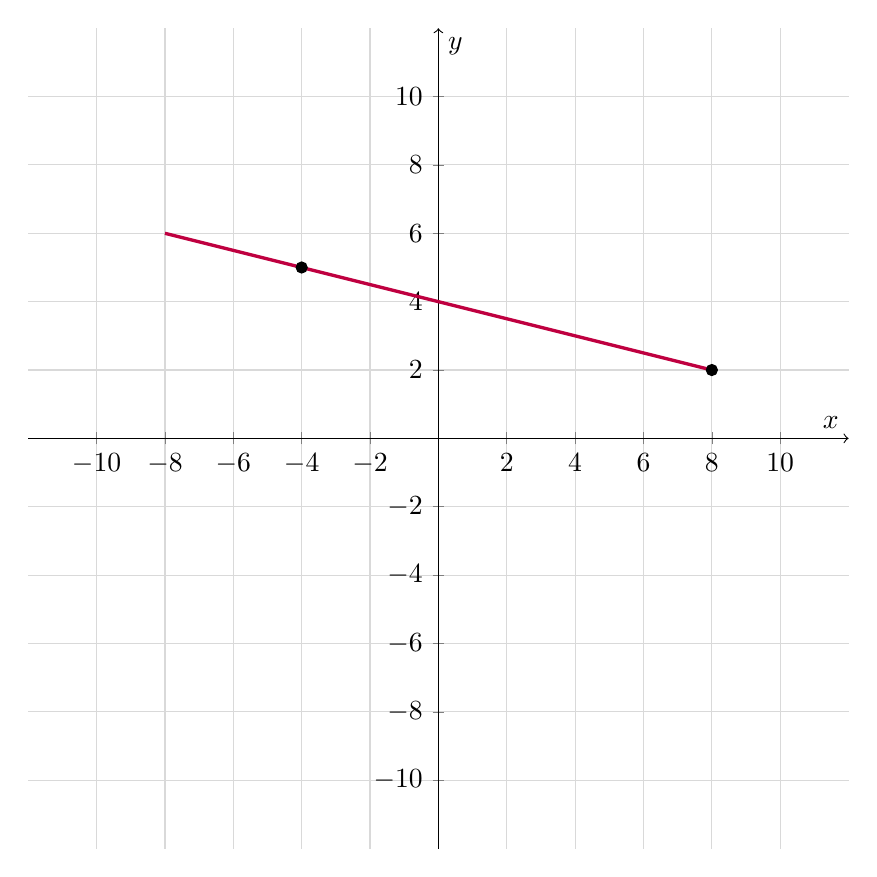
\begin{tikzpicture}[scale=1]
  \begin{axis}[
    axis lines=center,
    xmin=-10, xmax=10,
    ymin=-10, ymax=10,
    xtick={-10,-8,...,10},
    ytick={-10,-8,...,10},
    grid=both,
    width=12cm,
    height=12cm,
    enlargelimits=true,
    xlabel={$x$}, ylabel={$y$},
    ticks=both,
    every major grid/.style={gray!30},
    axis line style={->},
  ]
    % Plot the line
    \addplot[very thick, purple] coordinates {(-8,6) (8,2)};
    \filldraw [black] (-4,5) circle (2pt);
    \filldraw [black] (8,2) circle (2pt);
  \end{axis}
\end{tikzpicture}
\end{center}

If a new graph of three linear equations is created using the system of equations shown and the equation \( x + 4y = -16 \), how many solutions \( (x, y) \) will the resulting system of three equations have?

\vspace{0.75em}

\choicebox{A}{Zero}
\choicebox{B}{Exactly one}
\choicebox{C}{Exactly two}
\choicebox{D}{Infinitely many}


\newpage
\subsection*{1.5 Linear Inequality in One or Two Variables}
\vspace{0.5em}

\setcounter{questionnum}{0}


\noindent\markforreview

\vspace{1em}

Adam’s school is a 20-minute walk or a 5-minute bus ride away from his house. The bus runs once every 30 minutes, and the number of minutes, \( w \), that Adam waits for the bus varies between 0 and 30. Which of the following inequalities gives the values of \( w \) for which it would be faster for Adam to walk to school?

\vspace{0.75em}

\choicebox{A}{$w - 5 < 20$}
\choicebox{B}{$w - 5 > 20$}
\choicebox{C}{$w + 5 < 20$}
\choicebox{D}{$w + 5 > 20$}

\newpage

\noindent\markforreview

\vspace{1em}

A laundry service is buying detergent and fabric softener from its supplier. The supplier will deliver no more than 300 pounds in a shipment. Each container of detergent weighs 7.35 pounds, and each container of fabric softener weighs 6.2 pounds. The service wants to buy at least twice as many containers of detergent as containers of fabric softener. Let \( d \) represent the number of containers of detergent, and let \( s \) represent the number of containers of fabric softener, where \( d \) and \( s \) are nonnegative integers. Which of the following systems of inequalities best represents this situation?

\vspace{0.75em}

\choicebox{A}{$7.35d + 6.2s \leq 300$, \\ \hspace*{1.5em} $d \geq 2s$}
\choicebox{B}{$7.35d + 6.2s \leq 300$, \\ \hspace*{1.5em} $2d \geq s$}
\choicebox{C}{$14.7d + 6.2s \leq 300$, \\ \hspace*{1.5em} $d \geq 2s$}
\choicebox{D}{$14.7d + 6.2s \leq 300$, \\ \hspace*{1.5em} $2d \geq s$}

\newpage
\noindent\markforreview

\vspace{1em}

A local transit company sells a monthly pass for \$95 that allows an unlimited number of trips of any length. Tickets for individual trips cost \$1.50, \$2.50, or \$3.50, depending on the length of the trip. What is the minimum number of trips per month for which a monthly pass could cost less than purchasing individual tickets for trips?



\vspace{5em}

\noindent\markforreview

\vspace{1em}

Which point \( (x, y) \) is a solution to the given system of inequalities in the \( xy \)-plane?
\[
\begin{aligned}
y &\leq x + 7 \\
y &\geq -2x - 1
\end{aligned}
\]

\vspace{0.75em}

\choicebox{A}{$(-14, 0)$}
\choicebox{B}{$(0, -14)$}
\choicebox{C}{$(0, 14)$}
\choicebox{D}{$(14, 0)$}

\newpage
\noindent\markforreview

\vspace{1em}

A salesperson’s total earnings consist of a base salary of \( x \) dollars per year, plus commission earnings of 11\% of the total sales the salesperson makes during the year. This year, the salesperson has a goal for the total earnings to be at least 3 times and at most 4 times the base salary. Which of the following inequalities represents all possible values of total sales \( s \), in dollars, the salesperson can make this year in order to meet that goal?

\vspace{0.75em}

\choicebox{A}{$2x \leq s \leq 3x$}
\choicebox{B}{$\dfrac{2}{0.11}x \leq s \leq \dfrac{3}{0.11}x$}
\choicebox{C}{$3x \leq s \leq 4x$}
\choicebox{D}{$\dfrac{3}{0.11}x \leq s \leq \dfrac{4}{0.11}x$}

\vspace{2em}

\noindent\markforreview

\vspace{1em}

A number \( x \) is at most 2 less than 3 times the value of \( y \). If the value of \( y \) is \( -4 \), what is the greatest possible value of \( x \)?


\vspace{5em}

\noindent\markforreview

\vspace{1em}

A small business owner budgets \$2{,}200 to purchase candles. The owner must purchase a minimum of 200 candles to maintain the discounted pricing. If the owner pays \$4.90 per candle to purchase small candles and \$11.60 per candle to purchase large candles, what is the maximum number of large candles the owner can purchase to stay within the budget and maintain the discounted pricing?

\newpage

\noindent\markforreview

\vspace{1em}

A psychologist set up an experiment to study the tendency of a person to select the first item when presented with a series of items. In the experiment, 300 people were presented with a set of five pictures arranged in random order. Each person was asked to choose the most appealing picture. Of the first 150 participants, 36 chose the first picture in the set. Among the remaining 150 participants, $p$ people chose the first picture in the set. If more than 20\% of all participants chose the first picture in the set, which of the following inequalities best describes the possible values of $p$?

\vspace{0.75em}

\choicebox{A}{$p > 0.20(300 - 36),\ \text{where } p \leq 150$}
\choicebox{B}{$p > 0.20(300 + 36),\ \text{where } p \leq 150$}
\choicebox{C}{$p - 36 > 0.20(300),\ \text{where } p \leq 150$}
\choicebox{D}{$p + 36 > 0.20(300),\ \text{where } p \leq 150$}

\vspace{2em}

\noindent\markforreview

\vspace{1em}

The triangle inequality theorem states that the sum of any two sides of a triangle must be greater than the length of the third side. If a triangle has side lengths of $6$ and $12$, which inequality represents the possible lengths, $x$, of the third side of the triangle?

\vspace{0.75em}

\choicebox{A}{$x < 18$}
\choicebox{B}{$x > 18$}
\choicebox{C}{$6 < x < 18$}
\choicebox{D}{$x < 6 \text{ or } x > 18$}

\newpage
\noindent\markforreview

\vspace{1em}

The formula above is Ohm’s law for an electric circuit with current $I$, in amperes, potential difference $V$, in volts, and resistance $R$, in ohms.

\[
I = \frac{V}{R}
\]

A circuit has a resistance of $500$ ohms, and its potential difference will be generated by $n$ six-volt batteries that produce a total potential difference of $6n$ volts. If the circuit is to have a current of no more than $0.25$ ampere, what is the greatest number, $n$, of six-volt batteries that can be used?
\newpage

\noindent\markforreview

\vspace{1em}

For which of the following tables are all the values of \( x \) and their corresponding values of \( y \) solutions to the given inequality?
\[
y < 6x + 2
\]

\vspace{0.75em}

\choicebox{A}{
\[
\begin{array}{|c|c|}
\hline
x & y \\
\hline
3 & 20 \\
5 & 32 \\
7 & 44 \\
\hline
\end{array}
\]
}

\choicebox{B}{
\[
\begin{array}{|c|c|}
\hline
x & y \\
\hline
3 & 16 \\
5 & 36 \\
7 & 40 \\
\hline
\end{array}
\]
}

\choicebox{C}{
\[
\begin{array}{|c|c|}
\hline
x & y \\
\hline
3 & 16 \\
5 & 28 \\
7 & 40 \\
\hline
\end{array}
\]
}

\choicebox{D}{
\[
\begin{array}{|c|c|}
\hline
x & y \\
\hline
3 & 24 \\
5 & 36 \\
7 & 48 \\
\hline
\end{array}
\]
}

\newpage
\noindent\markforreview

\vspace{1em}

For which of the following tables are all the values of \( x \) and their corresponding values of \( y \) solutions to the given inequality?
\[
y > 13x - 18
\]

\vspace{0.75em}

\choicebox{A}{
\[
\begin{array}{|c|c|}
\hline
x & y \\
\hline
3 & 21 \\
5 & 47 \\
8 & 86 \\
\hline
\end{array}
\]
}

\choicebox{B}{
\[
\begin{array}{|c|c|}
\hline
x & y \\
\hline
3 & 26 \\
5 & 42 \\
8 & 86 \\
\hline
\end{array}
\]
}

\choicebox{C}{
\[
\begin{array}{|c|c|}
\hline
x & y \\
\hline
3 & 16 \\
5 & 42 \\
8 & 81 \\
\hline
\end{array}
\]
}

\choicebox{D}{
\[
\begin{array}{|c|c|}
\hline
x & y \\
\hline
3 & 26 \\
5 & 52 \\
8 & 91 \\
\hline
\end{array}
\]
}

\newpage
\noindent\markforreview

\vspace{1em}

A shipping service restricts the dimensions of the boxes it will ship for a certain type of service. The restriction states that for boxes shaped like rectangular prisms, the sum of the perimeter of the base of the box and the height of the box cannot exceed 130 inches. The perimeter of the base is determined using the width and length of the box. If a box has a height of 60 inches and its length is 2.5 times the width, which inequality shows the allowable width \( x \), in inches, of the box?

\vspace{0.75em}

\choicebox{A}{$0 < x \leq 10$}
\choicebox{B}{$0 < x \leq 11\frac{2}{3}$}
\choicebox{C}{$0 < x \leq 17\frac{1}{2}$}
\choicebox{D}{$0 < x \leq 20$}

\vspace{2em}

\noindent\markforreview

\vspace{1em}

A business owner plans to purchase the same model of chair for each of the 81 employees. The total budget to spend on these chairs is \$14,000, which includes a 7\% sales tax. Which of the following is closest to the maximum possible price per chair, before sales tax, the business owner could pay based on this budget?

\vspace{0.75em}

\choicebox{A}{\$148.15}
\choicebox{B}{\$161.53}
\choicebox{C}{\$172.84}
\choicebox{D}{\$184.94}

\newpage


\noindent\markforreview

\vspace{1em}

Ken is working this summer as part of a crew on a farm. He earned \$8 per hour for the first 10 hours he worked this week. Because of his performance, his crew leader raised his salary to \$10 per hour for the rest of the week. Ken saves 90\% of his earnings from each week. What is the least number of hours he must work the rest of the week to save at least \$270 for the week?

\vspace{0.75em}

\choicebox{A}{38}
\choicebox{B}{33}
\choicebox{C}{22}
\choicebox{D}{16}

\newpage
\noindent\markforreview


\[
\begin{aligned}
y &> 2x - 1 \\
2x &> 5
\end{aligned}
\]

Which of the following consists of the \( y \)-coordinates of all the points that satisfy the system of inequalities above?

\vspace{0.75em}

\choicebox{A}{$y > 6$}
\choicebox{B}{$y > 4$}
\choicebox{C}{$y > \frac{5}{2}$}
\choicebox{D}{$y > \frac{7}{2}$}





\end{document}
